% !TEX program = xelatex
% ============================================================================
% Arquitectura de microservicios por esquema
% Proyecto Final de Bases de Datos - Inventario, Compras y Ventas (PostgreSQL)
% ============================================================================
\documentclass[tikz, border=14pt]{standalone}

\usepackage{fontspec}
\setmainfont{STIX Two Text}
\setsansfont{Source Sans 3}[Scale=MatchLowercase]
\setmonofont{JetBrains Mono}[Scale=MatchLowercase]

\usetikzlibrary{arrows.meta, calc}

% ---------------------------------------------------------------- paleta
\definecolor{negro}{HTML}{1F2933}
\definecolor{gris}{HTML}{616E7C}
\definecolor{grisClaro}{HTML}{9AA5B1}
\definecolor{linea}{HTML}{D3DCE6}
\definecolor{fondo}{HTML}{F4F6F8}

\definecolor{cCat}{HTML}{2F6DB5}
\definecolor{cCom}{HTML}{C96800}
\definecolor{cInv}{HTML}{1E7A45}
\definecolor{cVen}{HTML}{A82010}
\definecolor{cIde}{HTML}{6030A0}
\definecolor{cRep}{HTML}{2C3E50}

% ---------------------------------------------------------------- estilos
\tikzset{
  card/.style={
    draw=linea, line width=0.6pt, fill=white,
    rounded corners=2pt
  },
  band/.style={
    draw=linea, line width=0.6pt, fill=fondo,
    rounded corners=2pt
  },
  rail/.style={
    draw=grisClaro, line width=0.6pt,
    dash pattern=on 3pt off 2.4pt
  },
  flow/.style={
    -{Stealth[length=4.2pt, width=3.2pt]},
    draw=gris, line width=0.7pt
  },
  biflow/.style={
    {Stealth[length=4.2pt, width=3.2pt]}-{Stealth[length=4.2pt, width=3.2pt]},
    draw=gris, line width=0.7pt
  },
  ref/.style={
    -{Stealth[length=3.4pt, width=2.6pt]},
    draw=grisClaro, line width=0.55pt,
    dash pattern=on 2.6pt off 2pt
  },
  rotulo/.style={
    font=\sffamily\fontsize{6.4}{7.4}\selectfont,
    text=gris
  }
}

% ---------------------------------------------------------------- macros
% \servicio{y}{color}{titulo}{esquema}{tablas}{rol}
\newcommand{\servicio}[6]{%
  \fill[#2] (0,#1) rectangle (0.13,#1-1.70);
  \draw[card] (0,#1) rectangle (12.80,#1-1.70);
  \node[anchor=north west,
        font=\sffamily\bfseries\fontsize{9.4}{11}\selectfont,
        text=negro] at (0.30,#1-0.24) {#3};
  \node[anchor=north east,
        font=\ttfamily\fontsize{6.8}{8}\selectfont,
        text=gris] at (12.62,#1-0.27) {esquema #4};
  \node[anchor=north west,
        font=\ttfamily\fontsize{6.2}{7.6}\selectfont,
        text=negro,
        text width=12.3cm, align=left] at (0.30,#1-0.78) {#5};
  \node[anchor=south west,
        font=\sffamily\fontsize{6.5}{7.6}\selectfont,
        text=gris] at (0.30,#1-1.70+0.14) {#6};
}

\begin{document}
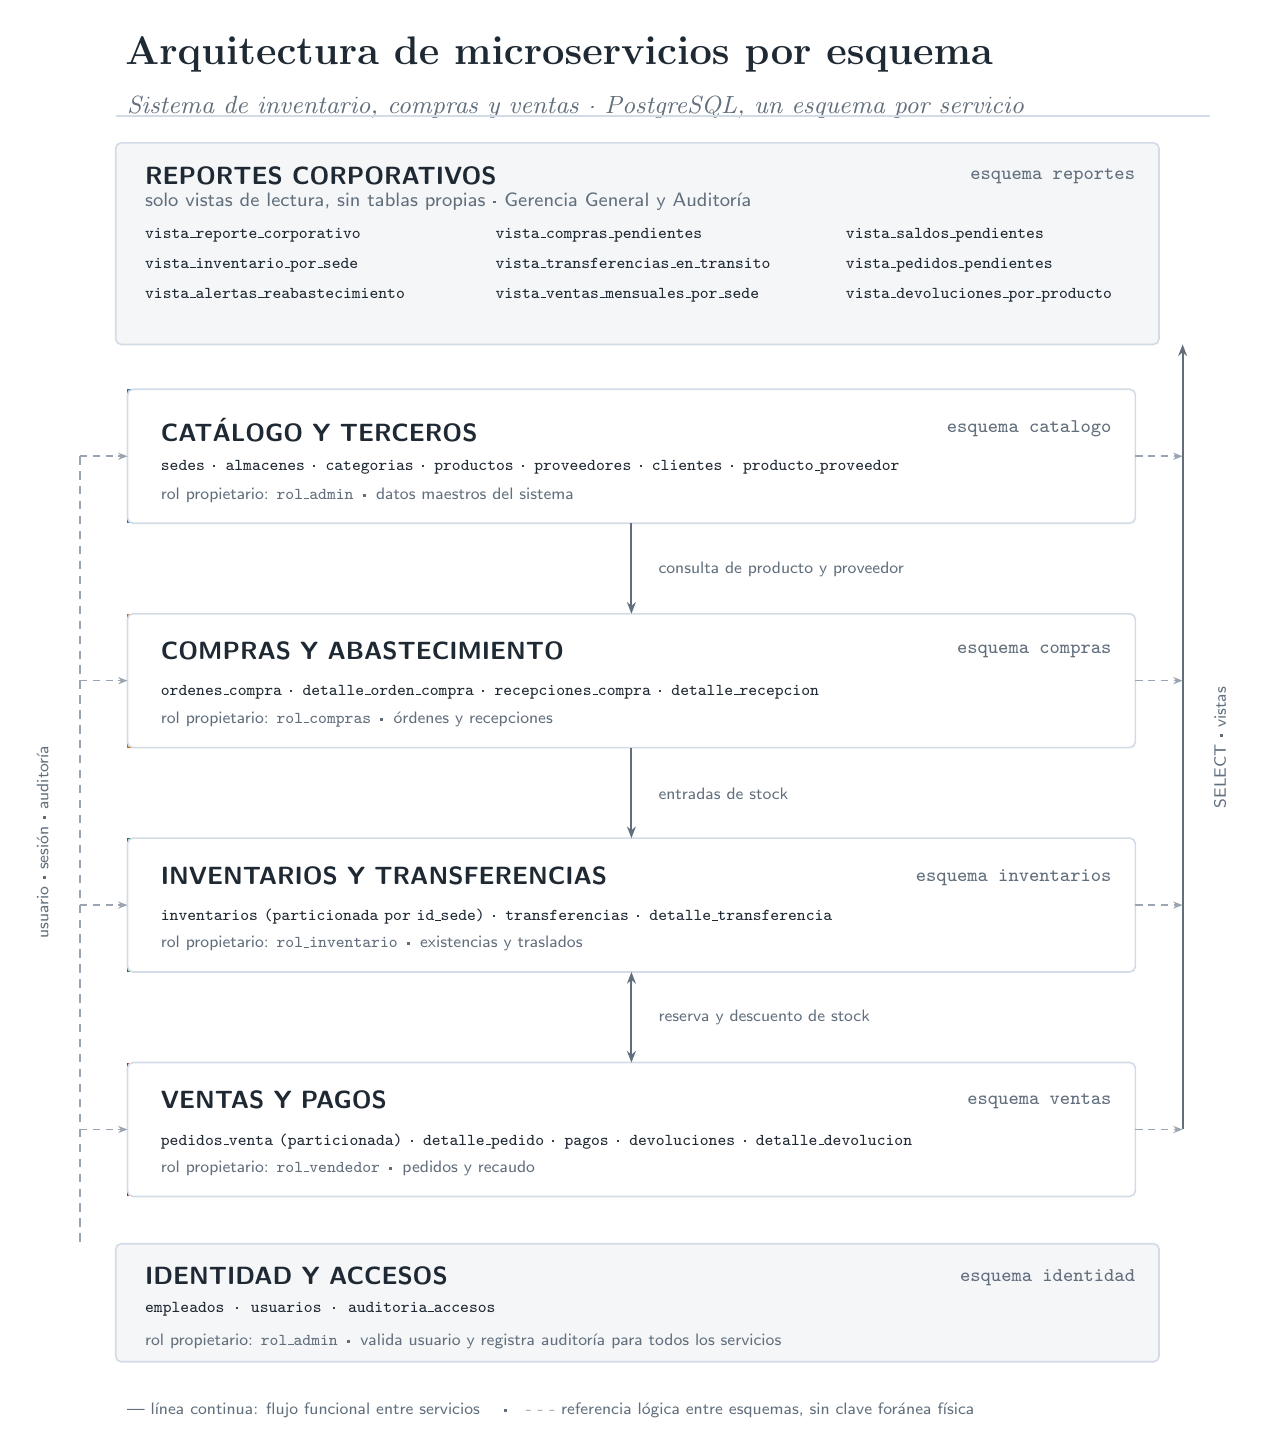
\begin{tikzpicture}

% ================================================================
% TITULO
% ================================================================
\node[anchor=north west,
      font=\bfseries\fontsize{15.5}{19}\selectfont,
      text=negro] at (-0.15,0.15)
  {Arquitectura de microservicios por esquema};
\node[anchor=north west,
      font=\itshape\fontsize{9}{11}\selectfont,
      text=gris] at (-0.13,-0.60)
  {Sistema de inventario, compras y ventas \textperiodcentered{}
   PostgreSQL, un esquema por servicio};
\draw[linea, line width=0.6pt] (-0.15,-0.98) -- (13.75,-0.98);

% ================================================================
% CAPA DE REPORTES
% ================================================================
\draw[band] (-0.15,-1.32) rectangle (13.10,-3.88);
\node[anchor=north west,
      font=\sffamily\bfseries\fontsize{9.4}{11}\selectfont,
      text=negro] at (0.10,-1.50) {REPORTES CORPORATIVOS};
\node[anchor=north east,
      font=\ttfamily\fontsize{6.8}{8}\selectfont,
      text=gris] at (12.92,-1.53) {esquema reportes};
\node[anchor=north west,
      font=\sffamily\fontsize{6.6}{7.8}\selectfont,
      text=gris] at (0.10,-1.83)
  {solo vistas de lectura, sin tablas propias
   \textperiodcentered{} Gerencia General y Auditor\'ia};

% vistas en tres columnas
\foreach \dx/\vista in {%
  0.10/{vista\_reporte\_corporativo},
  4.55/{vista\_compras\_pendientes},
  9.00/{vista\_saldos\_pendientes}} {%
  \node[anchor=north west,
        font=\ttfamily\fontsize{6.1}{8}\selectfont,
        text=negro] at (\dx,-2.28) {\vista};
}
\foreach \dx/\vista in {%
  0.10/{vista\_inventario\_por\_sede},
  4.55/{vista\_transferencias\_en\_transito},
  9.00/{vista\_pedidos\_pendientes}} {%
  \node[anchor=north west,
        font=\ttfamily\fontsize{6.1}{8}\selectfont,
        text=negro] at (\dx,-2.66) {\vista};
}
\foreach \dx/\vista in {%
  0.10/{vista\_alertas\_reabastecimiento},
  4.55/{vista\_ventas\_mensuales\_por\_sede},
  9.00/{vista\_devoluciones\_por\_producto}} {%
  \node[anchor=north west,
        font=\ttfamily\fontsize{6.1}{8}\selectfont,
        text=negro] at (\dx,-3.04) {\vista};
}

% ================================================================
% SERVICIOS (columna central, de arriba hacia abajo)
% ================================================================
\servicio{-4.45}{cCat}{CAT\'ALOGO Y TERCEROS}{catalogo}
  {sedes \textperiodcentered{} almacenes \textperiodcentered{}
   categorias \textperiodcentered{} productos \textperiodcentered{}
   proveedores \textperiodcentered{} clientes \textperiodcentered{}
   producto\_proveedor}
  {rol propietario: \texttt{rol\_admin}\enspace\textperiodcentered\enspace
   datos maestros del sistema}

\servicio{-7.30}{cCom}{COMPRAS Y ABASTECIMIENTO}{compras}
  {ordenes\_compra \textperiodcentered{} detalle\_orden\_compra
   \textperiodcentered{} recepciones\_compra \textperiodcentered{}
   detalle\_recepcion}
  {rol propietario: \texttt{rol\_compras}\enspace\textperiodcentered\enspace
   \'ordenes y recepciones}

\servicio{-10.15}{cInv}{INVENTARIOS Y TRANSFERENCIAS}{inventarios}
  {inventarios (particionada por id\_sede) \textperiodcentered{}
   transferencias \textperiodcentered{} detalle\_transferencia}
  {rol propietario: \texttt{rol\_inventario}\enspace\textperiodcentered\enspace
   existencias y traslados}

\servicio{-13.00}{cVen}{VENTAS Y PAGOS}{ventas}
  {pedidos\_venta (particionada) \textperiodcentered{}
   detalle\_pedido \textperiodcentered{} pagos \textperiodcentered{}
   devoluciones \textperiodcentered{} detalle\_devolucion}
  {rol propietario: \texttt{rol\_vendedor}\enspace\textperiodcentered\enspace
   pedidos y recaudo}

% ================================================================
% FLUJO FUNCIONAL ENTRE SERVICIOS
% ================================================================
\draw[flow] (6.40,-6.15) -- (6.40,-7.30);
\node[anchor=west, rotulo] at (6.62,-6.73)
  {consulta de producto y proveedor};

\draw[flow] (6.40,-9.00) -- (6.40,-10.15);
\node[anchor=west, rotulo] at (6.62,-9.58)
  {entradas de stock};

\draw[biflow] (6.40,-11.85) -- (6.40,-13.00);
\node[anchor=west, rotulo] at (6.62,-12.43)
  {reserva y descuento de stock};

% ================================================================
% RIEL DE IDENTIDAD (izquierda)
% ================================================================
\draw[rail] (-0.60,-5.30) -- (-0.60,-15.30);
\foreach \y in {-5.30,-8.15,-11.00,-13.85} {%
  \draw[ref] (-0.60,\y) -- (0,\y);
}
\node[rotate=90, anchor=south, rotulo] at (-0.88,-10.20)
  {usuario \textperiodcentered{} sesi\'on \textperiodcentered{} auditor\'ia};

% ================================================================
% RIEL DE REPORTES (derecha)
% ================================================================
\draw[flow] (13.40,-13.85) -- (13.40,-3.88);
\foreach \y in {-5.30,-8.15,-11.00,-13.85} {%
  \draw[ref] (12.80,\y) -- (13.40,\y);
}
\node[rotate=90, anchor=north, rotulo] at (13.68,-9.00)
  {SELECT \textperiodcentered{} vistas};

% ================================================================
% CAPA DE IDENTIDAD
% ================================================================
\draw[band] (-0.15,-15.30) rectangle (13.10,-16.80);
\node[anchor=north west,
      font=\sffamily\bfseries\fontsize{9.4}{11}\selectfont,
      text=negro] at (0.10,-15.47) {IDENTIDAD Y ACCESOS};
\node[anchor=north east,
      font=\ttfamily\fontsize{6.8}{8}\selectfont,
      text=gris] at (12.92,-15.50) {esquema identidad};
\node[anchor=north west,
      font=\ttfamily\fontsize{6.2}{7.6}\selectfont,
      text=negro] at (0.10,-15.92)
  {empleados \textperiodcentered{} usuarios \textperiodcentered{}
   auditoria\_accesos};
\node[anchor=north west,
      font=\sffamily\fontsize{6.5}{7.6}\selectfont,
      text=gris] at (0.10,-16.32)
  {rol propietario: \texttt{rol\_admin}\enspace\textperiodcentered\enspace
   valida usuario y registra auditor\'ia para todos los servicios};

% ================================================================
% LEYENDA
% ================================================================
\node[anchor=north west,
      font=\sffamily\fontsize{6.4}{8}\selectfont,
      text=gris] at (-0.13,-17.20)
  {\textcolor{gris}{---} l\'inea continua: flujo funcional entre servicios
   \quad\textperiodcentered\quad
   \textcolor{grisClaro}{- - -} referencia l\'ogica entre esquemas, sin clave
   for\'anea f\'isica};

\end{tikzpicture}
\end{document}
